\documentclass{article}
\usepackage{ctex}
\usepackage{graphicx}
\usepackage{listings}
\usepackage{xcolor}

\title{深度学习与神经网络第一次课程项目}
\author{王逸群 19307110397}
\date{2022.3}

\definecolor{gray}{rgb}{0.99,0.99,0.99}

\lstdefinestyle{mystyle}{
	basicstyle=\footnotesize,
	backgroundcolor=\color{gray},
	numbers=left
}

\lstset{style=mystyle}

\begin{document}

\maketitle

目标:
对输入的$ 16 \times 16 $手写数字灰度图进行识别;

数据集:存储于\verb|data.mat|;

激活函数:Tanh函数;

损失函数:平方损失函数;

优化方法:随机梯度下降法。

模型评估:
在测试集上的错误率为47\%,
在验证集上的错误率如图\ref{fig:0}。

\begin{figure}[h]
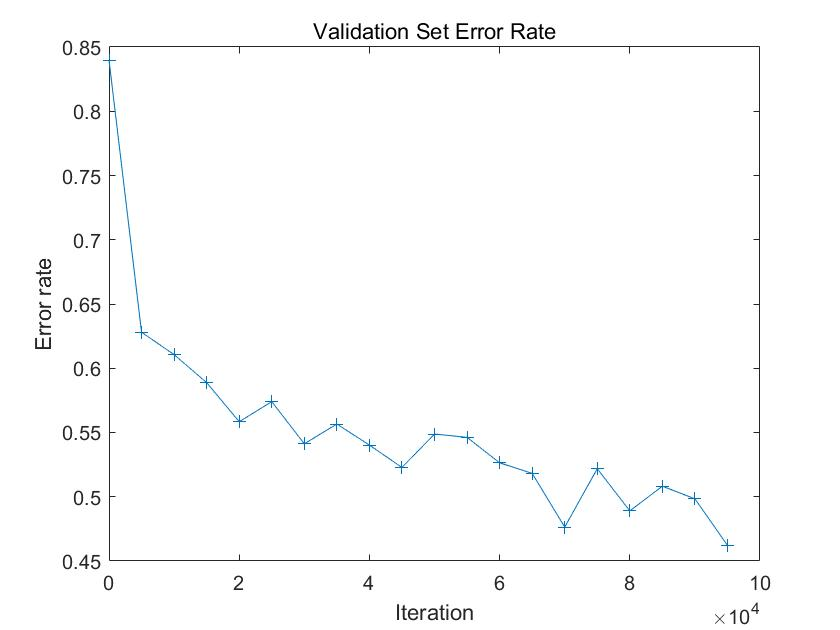
\includegraphics[width=\textwidth]{0.jpg}
\caption{原始模型在验证集上的错误率}
\label{fig:0}
\end{figure}

\section{网络结构}

程序中,
变量\verb|nHidden|为一个向量,
其维度表示网络隐藏层的个数,
各个分量表示每个隐藏层的神经元个数。

基础模型中,\verb|nHidden = 10|,
将其修改得到的验证集和测试集错误率
如图\ref{fig:1}和表\ref{table:1}所示。

\begin{figure}[h]
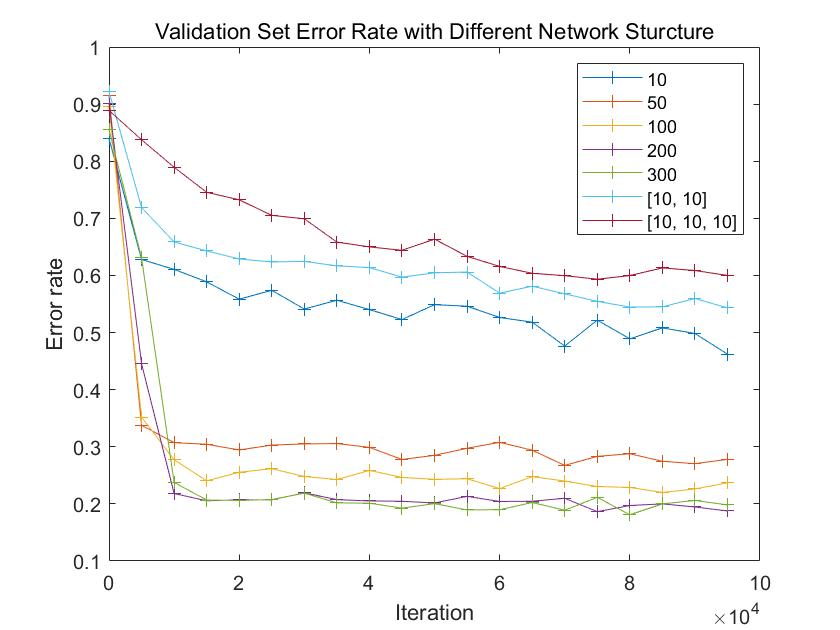
\includegraphics[width=\textwidth]{1.jpg}
\caption{不同网络结构的模型在验证集上的错误率}
\label{fig:1}
\end{figure}

\begin{table}[h]
\centering
\begin{tabular}{|l|l|} 
\hline
网络结构 & 测试集错误率 \\
\hline
\verb|nHidden = 10| & 0.470 \\
\verb|nHidden = 50| & 0.255 \\
\verb|nHidden = 100| & 0.228 \\
\verb|nHidden = 200| & 0.181 \\
\verb|nHidden = 300| & 0.177\\
\verb|nHidden = [10, 10]| & 0.536 \\
\verb|nHidden = [10, 10, 10]| & 0.562 \\
\hline
\end{tabular}
\caption{不同网络结构的模型在测试集上的错误率}
\label{table:1}
\end{table}

可以看到,
随着单层网络神经元个数的增加,
模型在测试集上的错误率逐渐减小,
但是减小的程度趋缓。
鉴于训练模型的时间成本随着网络神经元个数的增加而增加,
神经元个数的选取是精度与成本的权衡。

另一方面,
随着网络隐藏层个数的增加,
模型在测试集上的错误率逐渐增加,
可能的原因是较深的网络难以优化。

\section{学习率与Momentum}

在基础模型中,
学习率始终为\verb|alpha = 1e-3|,
且没有引入Momentum。
本节尝试使用
修改学习率常数、
学习率衰减、
引入Momentum
的方式来改进模型,
得到的验证集和测试集错误率
如图\ref{fig:2}和表\ref{table:2}所示。

\begin{figure}[h]
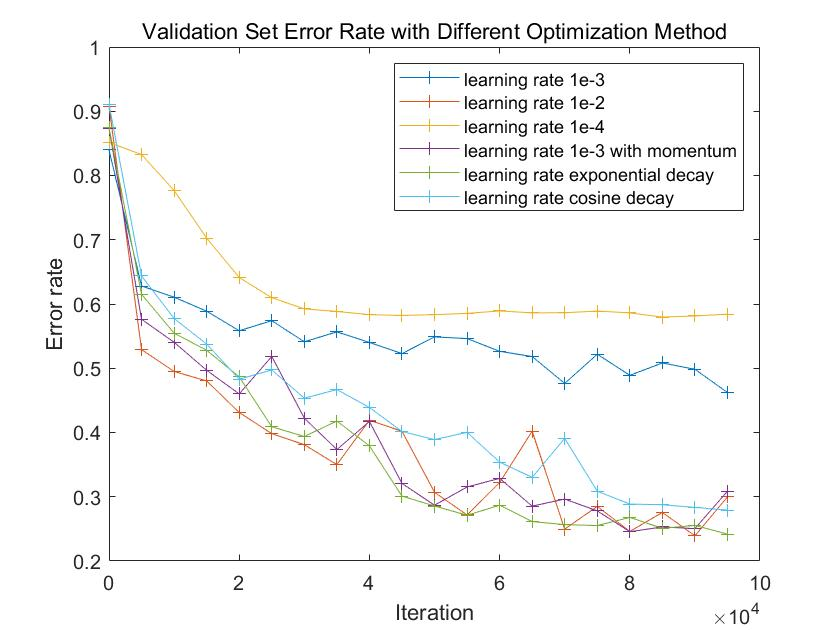
\includegraphics[width=\textwidth]{2.jpg}
\caption{采用不同优化方式的模型在验证集上的错误率}
\label{fig:2}
\end{figure}

\begin{table}[h]
\centering
\begin{tabular}{|l|l|l|l|} 
\hline
初始学习率 & 学习率衰减 & Momentum & 测试集错误率 \\
\hline
\verb|alpha = 1e-3| & 无 & 无 & 0.470 \\
\verb|alpha = 1e-2| & 无 & 无 & 0.267\\
\verb|alpha = 1e-4| & 无 & 无 & 0.584\\
\verb|alpha = 1e-3| & 无 & 0.9 & 0.322\\
\verb|alpha = 1e-2| & 指数衰减 & 无 & 0.277 \\
\verb|alpha = 1e-2| & 余弦衰减 & 无 & 0.259 \\
\hline
\end{tabular}
\caption{不同学习方式的模型在测试集上的错误率}
\label{table:2}
\end{table}

可以看到,
随着常数学习率的增加,
验证集错误率的收敛速度变快,
但是错误率变得越发不稳定。
为了解决这个问题,
采用指数衰减和余弦衰减两种学习率衰减方式,
两者效果相近。

另一方面,
使用Momenteum也能改进模型的训练效果。

\section{损失函数计算}

基础模型中,
在计算损失函数时,
使用了矩阵计算,
而非以下标作为循环变量的循环计算,
并且避免进行不必要的条件判断。
如反向传播算法:

\begin{lstlisting}
% output layer
error = 2 * error;
gradOutput = gradOutput + Activation{end}' * error;
error = sech(netActivation{end}) .^ 2 .* ...
    (error * weightsOutput');
% hidden layers
for indexHidden = length(nHidden) - 1: -1: 1
    gradHidden{indexHidden} = gradHidden{indexHidden} + ...
        Activation{indexHidden}' * error;
    error = sech(netActivation{indexHidden}) .^ 2 .*  ...
        (error * weightsHidden{indexHidden}');
end
% input layer
gradInput = gradInput + X(indexInput,:)' * error;
\end{lstlisting}

其中,
\verb|error|表示误差项,初始值是模型输出值与真实值的差;

\section{正则化}

基础模型中,没有加入正则化。
本节尝试调整正则化参数来改进模型,
得到的验证集和测试集错误率
如图\ref{fig:4}和表\ref{table:4}所示。

\begin{figure}[h]
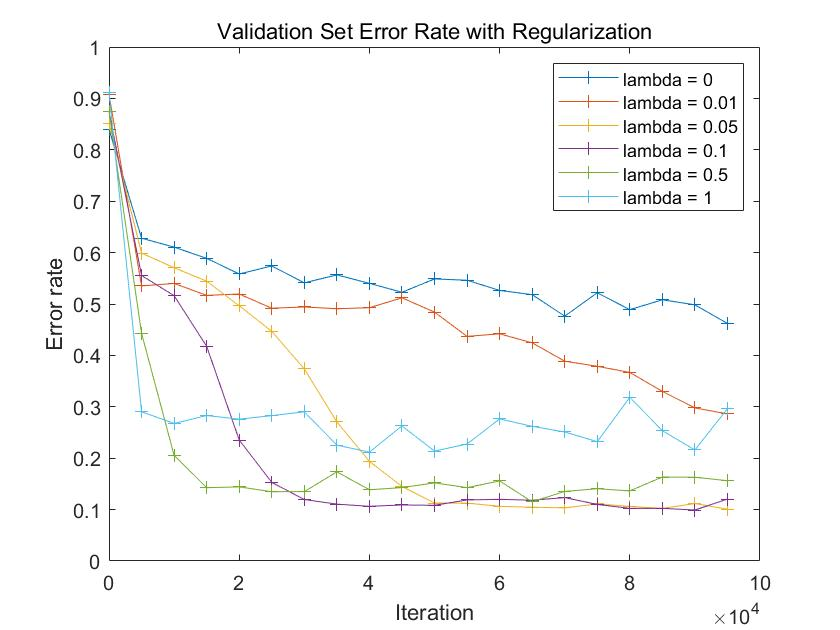
\includegraphics[width=\textwidth]{4.jpg}
\caption{不同正则化参数的模型在验证集上的错误率}
\label{fig:4}
\end{figure}

\begin{table}[p]
\centering
\begin{tabular}{|l|l|} 
\hline
正则化参数 & 测试集错误率 \\
\hline
0 & 0.470 \\
0.01 & 0.286 \\
0.05 & 0.104 \\
0.1 & 0.100 \\
0.5 & 0.164 \\
1 & 0.235 \\
\hline
\end{tabular}
\caption{不同正则化参数的模型在测试集上的错误率}
\label{table:4}
\end{table}

可以看到,
正则化参数为0.05时,
正则化效果还不明显。
之后,
随着正则化参数的增加,
验证集错误率的收敛速度变快,
但是错误率也变大。

\section{交叉熵损失函数}

基础模型中,损失函数是平方损失函数。
本节尝试加入Softmax函数、使用交叉熵损失函数来改进模型,
得到的验证集和测试集错误率
如图\ref{fig:5}和表\ref{table:5}所示。

\begin{figure}[p]
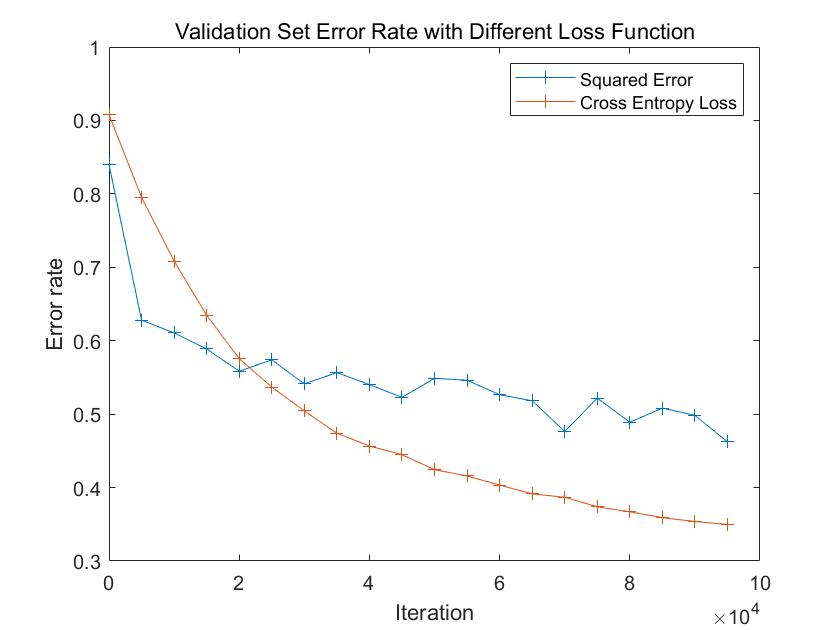
\includegraphics[width=\textwidth]{5.jpg}
\caption{不同损失函数的模型在验证集上的错误率}
\label{fig:5}
\end{figure}

\begin{table}[p]
\centering
\begin{tabular}{|l|l|} 
\hline
损失函数 & 测试集错误率 \\
\hline
平方损失函数 & 0.470 \\
交叉熵损失函数 & 0.353 \\
\hline
\end{tabular}
\caption{不同损失函数的模型在测试集上的错误率}
\label{table:5}
\end{table}

可以看到,
使用交叉熵损失函数会减小模型的错误率,
增加模型的稳定性,
但也会减小收敛速度。

\section{偏置}

基础模型中,输入带有偏置项,但隐藏层中没有。
本节使得每个隐藏层中的一个神经元成为偏置项,
以此来改进模型,
得到的验证集和测试集错误率
如图\ref{fig:6}和表\ref{table:6}所示。

\begin{figure}[h]
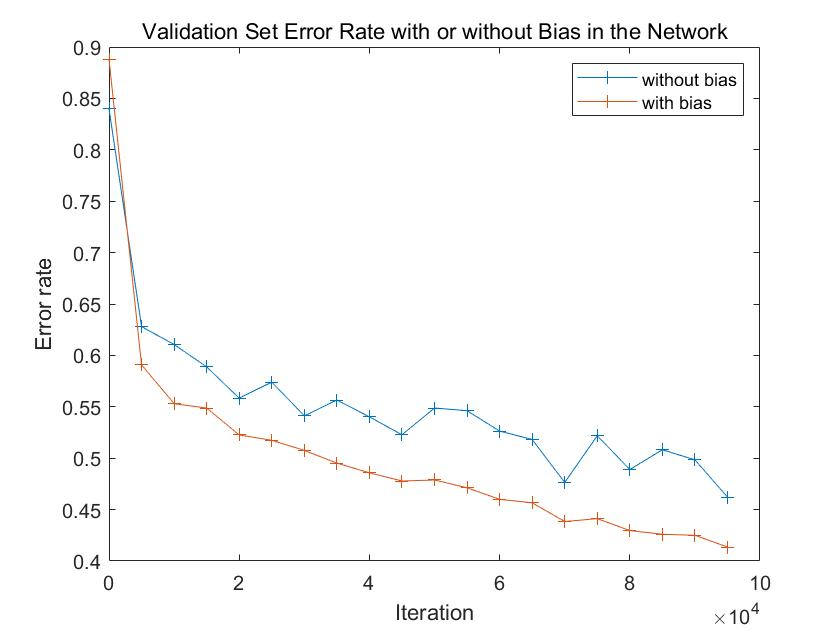
\includegraphics[width=\textwidth]{6.jpg}
\caption{不同偏置设置的模型在验证集上的错误率}
\label{fig:6}
\end{figure}

\begin{table}[h]
\centering
\begin{tabular}{|l|l|} 
\hline
隐藏层是否带有偏置 & 测试集错误率 \\
\hline
否 & 0.470 \\
是 & 0.372 \\
\hline
\end{tabular}
\caption{不同偏置设置的模型在测试集上的错误率}
\label{table:6}
\end{table}

可以看到,
隐藏层带有偏置会减小模型的错误率,
增加模型的稳定性。

\section{丢弃法}

本节使用丢弃法来改进模型,
即训练过程中,隐藏层中的神经元有一个固定的概率会被丢弃。
以此得到的验证集和测试集错误率
如图\ref{fig:7}和表\ref{table:7}所示。

\begin{figure}[h]
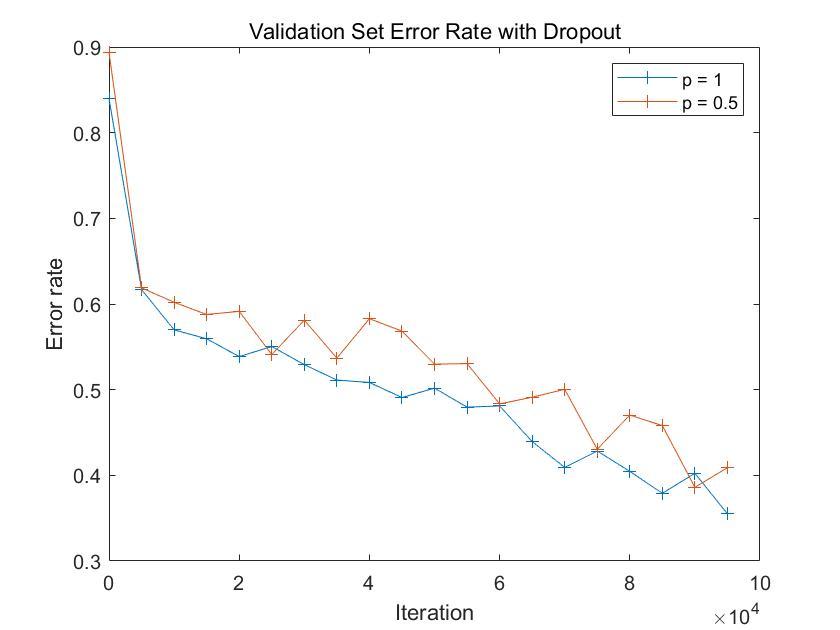
\includegraphics[width=\textwidth]{7.jpg}
\caption{使用丢弃法的模型在验证集上的错误率}
\label{fig:7}
\end{figure}

\begin{table}[h]
\centering
\begin{tabular}{|l|l|} 
\hline
神经元保留概率 & 测试集错误率 \\
\hline
1.0 & 0.348 \\
0.5 & 0.430 \\
\hline
\end{tabular}
\caption{使用丢弃法的模型在测试集上的错误率}
\label{table:7}
\end{table}

可以看到,
使用丢弃法对模型没有明显的改进。

\section{精调}

本节使用精调来改进模型,
即最后固定输入层和隐藏层的参数,
使用最小二乘法求解输出层的参数。
精调后,测试集错误率降至0.466。

\section{数据增强}

本节使用平移、旋转、调整大小等数据增强方法来改进模型。
具体的操作方法是,
对计算损失函数和梯度的函数增加一个参数\verb|prob|,
它是一个三维向量,
第一个维度表示图像平移的概率,
第二个维度表示图像旋转的概率,
第二个维度表示调整图像大小的概率。

若一张图像需要进行平移,
则平移的量服从标准正态分布,
空缺的像素点由正态分布填充。
若一张图像需要进行旋转,
则旋转的量服从方差为10的正态分布。
若一张图像需要调整大小,
则放大的倍数服从取值于1至1.1的均匀分布,
并裁剪其中$ 16 \times 16 $的区域。

最后得到的验证集和测试集错误率
如图\ref{fig:9}和表\ref{table:9}所示。

\begin{figure}[p]
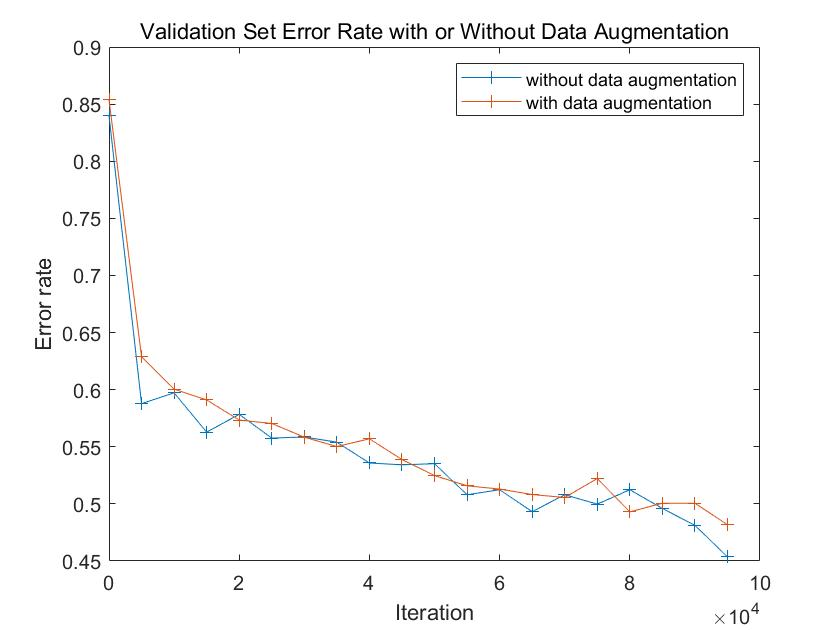
\includegraphics[width=\textwidth]{9.jpg}
\caption{使用数据增强的模型在验证集上的错误率}
\label{fig:9}
\end{figure}

\begin{table}[h]
\centering
\begin{tabular}{|l|l|} 
\hline
数据增强概率 & 测试集错误率 \\
\hline
0.0 & 0.469 \\
0.5 & 0.466 \\
\hline
\end{tabular}
\caption{使用数据增强的模型在测试集上的错误率}
\label{table:9}
\end{table}

可以看到,
使用数据增强对模型没有明显的改进,
但是会大幅降低模型训练速度。

\section{卷积}

本节通过在输入层使用卷积来改进模型,
以此得到的验证集和测试集错误率
如图\ref{fig:10}和表\ref{table:10}所示。

\begin{figure}[h]
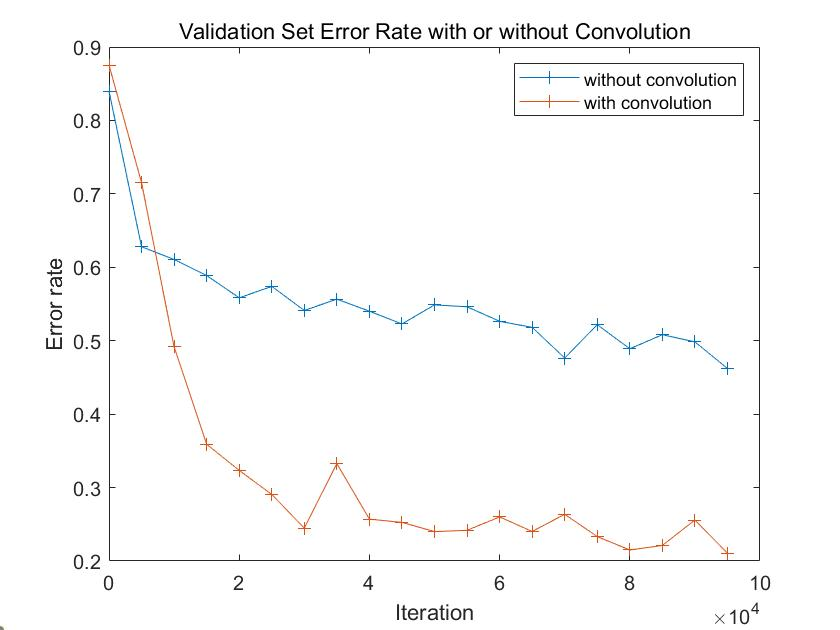
\includegraphics[width=\textwidth]{10.jpg}
\caption{使用卷积的模型在验证集上的错误率}
\label{fig:10}
\end{figure}

\begin{table}[h]
\centering
\begin{tabular}{|l|l|} 
\hline
是否使用卷积 & 测试集错误率 \\
\hline
否 & 0.470 \\
是 & 0.218 \\
\hline
\end{tabular}
\caption{使用卷积的模型在测试集上的错误率}
\label{table:10}
\end{table}

可以看到,使用卷积对模型的错误率有明显的改进。

\section{总结}

最终选择从三个方面改进模型:
首先,在输出层使用Softmax函数,并使用交叉熵损失函数;
其次,在输入层使用$ 5 \times 5 $的卷积核;
最后,使用正则化,系数为0.05。
改进后的模型在测试集上的错误率为7\%,
在验证集上的错误率如图\ref{fig:11}。

\begin{figure}[h]
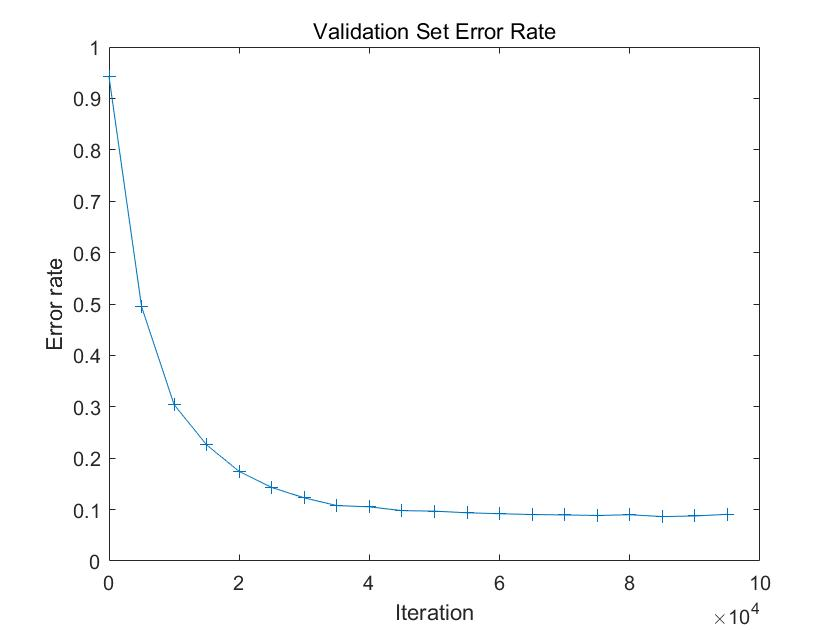
\includegraphics[width=\textwidth]{11.jpg}
\caption{改进后的模型在验证集上的错误率}
\label{fig:11}
\end{figure}

\end{document}